\documentclass[conference]{IEEEtran}
\IEEEoverridecommandlockouts
\usepackage{cite}
\usepackage{amsmath,amssymb,amsfonts}
\usepackage{graphicx}
\usepackage{textcomp}
\usepackage{xcolor}
\usepackage{booktabs}
\usepackage{url}

\def\BibTeX{{\rm B\kern-.05em{\sc i\kern-.025em b}\kern-.08em
    T\kern-.1667em\lower.7ex\hbox{E}\kern-.125emX}}

\begin{document}

\title{ASTRA: Adaptive Satellite Task and Resource Allocator for LEO Earth Observation\\
\thanks{This work was developed for the IEEE IAS Tunisia Annual Meeting (IASTAM 6.0) Technical Challenge in collaboration with the Tunisian Space Association (TUNSA).}
}

\author{
\IEEEauthorblockN{Mohamed Habib Abid\IEEEauthorrefmark{1}, Meriem Neffeti\IEEEauthorrefmark{1}}
\IEEEauthorblockA{\textit{Team IASTAM-OrbitEdge --- [confirm official team and institution names]} \\
Tunisia \\
Email: [confirm author email addresses]
\thanks{\IEEEauthorrefmark{1}Equal contribution.}
}
}

\maketitle

\begin{abstract}
Small Earth-observation satellites capture multispectral and Synthetic Aperture Radar data under intermittent contact and constrained onboard resources. We introduce ASTRA (Adaptive Satellite Task and Resource Allocator), a research prototype for the IASTAM 6.0 ``Process or Transmit?'' problem. Its current experiments evaluate a seeded, one-second-step LEO simulator and an implemented threshold heuristic. Across five four-orbit episodes (seeds 42--46), the heuristic achieved a mean delivered-utility ratio of 0.0283 (sample standard deviation 0.0024; 95\% t interval 0.0252--0.0313) and completed 1.53\% of generated payloads. Mean modeled energy draw was 291.41 kJ, mean battery state of charge stayed above the 30\% floor, and no safe-mode entry occurred. In a separate two-orbit trace (seed 42), simulated chip temperature reached 52.48$^\circ$C; the simulator throttles compute at 50$^\circ$C but does not enforce a hard temperature cap. Learned-policy, Lyapunov-scheduler, oracle, and hardware-calibration studies remain future work.
\end{abstract}

\begin{IEEEkeywords}
orbital edge computing, onboard task scheduling, energy- and thermal-aware computing, Lyapunov optimization, reinforcement learning, Low Earth Orbit, fault tolerance.
\end{IEEEkeywords}

\section{Introduction}
The 2026 edition of the IEEE IAS Tunisia Annual Meeting (IASTAM 6.0) Technical Challenge, organized in collaboration with the Tunisian Space Association (TUNSA), addresses an operational bottleneck in Earth-observation data handling. Orbital edge computing has drawn attention as a way to move selected processing closer to sensors \cite{denby2020orbital, suncatcher2025}. Google's Project Suncatcher is a proposed space-based AI infrastructure concept, not an operational orbital testbed \cite{suncatcher2025}.

Within this domain, Problem~1 (``Process or Transmit?'') targets an acute bottleneck in Earth Observation (EO): small satellites continuously capture high-resolution optical and Synthetic Aperture Radar (SAR) payloads (generating multi-megabyte payloads every $15\text{ s}$), yet operate under three binding physical constraints:
\begin{enumerate}
    \item \textbf{Battery Floor:} The simulator models a $100\text{ Wh}$ battery and clamps its state at a 30\% minimum depth-of-discharge floor.
    \item \textbf{Thermal Constraint:} Vacuum requires radiative heat rejection. The current simulator uses a first-order thermal proxy and pauses compute at 50$^\circ$C; it does not enforce a hard cap, and the measured trace reaches 52.48$^\circ$C.
    \item \textbf{Severe Downlink Bandwidth Choke:} Line-of-sight contact with ground stations is limited to short windows ($120\text{--}180\text{ s}$ per 90-minute orbit, about 2.8\% mean contact duty cycle) with an X-band rate of $20.0\text{ Mbps}$ ($2.5\text{ MB/s}$).
\end{enumerate}

For every captured payload, the onboard system must choose among four actions: PROCESS\_NOW (compression vs. inference), STORE\_QUEUE (time-shifted execution in Mass Memory Unit, MMU), TRANSMIT\_RAW (downlink during line-of-sight passes), or DISCARD\_DROP (pruning low-utility or cloud-occluded data). The optimization objective is to maximize cumulative scientific and operational utility, which decays exponentially over latency.

\textbf{Contributions:}
\begin{itemize}
    \item We characterize the repository's seeded one-second simulator and implemented multi-threshold heuristic.
    \item We report five four-orbit heuristic episodes with decision quality, task completion, energy, latency, MMU/RAM utilization, SEU counts, and safe-mode events.
    \item We identify an observed temperature excursion above the code's 50$^\circ$C throttling threshold, a limitation that motivates thermal-model and safety-guard validation.
\end{itemize}

\section{Related Work}
\subsection{Orbital and Edge Computing Systems}
Orbital edge computing surveys describe the systems-level case for in-space processing \cite{denby2020orbital}. Trabant is a recent serverless architecture proposal \cite{pfandzelter2024trabant}; the Tiansuan constellation provides a cloud-native satellite case study \cite{zhang2023satellite}. Broader treatments of Space AI \cite{chen2025spaceai} and Earth-observation image processing \cite{duggan2025advancing} provide context on onboard classification and inference. FPGA accelerator surveys \cite{lentaris2024fpga} and work on when to compute in space \cite{denby2025when} inform the modeled trade-offs; the simulator's numerical parameters remain assumptions rather than transferred empirical measurements.

\subsection{Control and Scheduling Paradigms}
Resource-constrained orbital scheduling is addressed via two dominant paradigms:
\begin{enumerate}
    \item \textbf{Lyapunov Optimization \& Drift-Plus-Penalty:} Prior work \cite{neely2010stochastic} motivates online scheduling; implementing and evaluating an orbital scheduler remains planned work.
    \item \textbf{Constrained Reinforcement Learning (CMDP):} The repository includes a Gymnasium environment; policy training and safety evaluation are not reported here.
\end{enumerate}

\subsection{Added Value of This Work}
Prior work motivates orbital edge processing and constrained scheduling. This interim study contributes a reproducible characterization of the current heuristic and identifies model and benchmarking gaps.

\section{Methodology}

\subsection{Physical Models \& Orbital Mechanics}
The satellite orbital environment and hardware state at time $t$ are formalized in Table~\ref{tab:system_params}.

\begin{table}[htbp]
\caption{Primary System and State Variables}
\label{tab:system_params}
\centering
\resizebox{\columnwidth}{!}{%
\begin{tabular}{llr}
\toprule
\textbf{Symbol} & \textbf{Physical Definition} & \textbf{Nominal Value / Range} \\
\midrule
$\tau_{\text{orbit}}, \tau_{\text{sun}}$ & Orbit period / Sunlit duration & $5400\text{ s}$ / $3300\text{ s}$ (90 / 55 min) \\
$P_{\text{harvest}}(t)$ & Solar power harvested & $0.0\text{ W}$ (ecl) to $30.0\text{ W}$ peak \\
$\text{SoC}(t)$ & Battery State-of-Charge & Floor $\ge 0.30$, Cap: $100.0\text{ Wh}$ \\
$T_{\text{chip}}(t)$ & Processor temperature & Ambient $0^\circ\text{C}$, Ceiling $\le 50.0^\circ\text{C}$ \\
$G(t)$ & Ground station contact flag & $\{0, 1\}$, $120\text{--}180\text{ s}$ pass (about 2.8\% mean duty) \\
$B_{\text{downlink}}$ & RF communication speed & $20.0\text{ Mbps} = 2.5\text{ MB/s}$ ($15.0\text{ W}$) \\
$p_{\text{seu}}$ & SEU bit-flip rate & $10^{-5}\text{ s}^{-1}$ cosmic radiation \\
$M_{\text{mmu}}, M_{\text{ram}}$ & Mass Memory / RAM & $32\,000\text{ MB}$ / $4\,000\text{ MB}$ \\
\bottomrule
\end{tabular}%
}
\end{table}

\subsubsection{Power and Battery Dynamics}
The simulator uses a 55-minute sunlight interval followed by a 35-minute eclipse. In sunlight, harvested power follows a sine-shaped profile from a 22.5 W base to a 30 W peak, with 30 s cosine tapers at sunlight boundaries; eclipse harvesting is zero.

Battery energy is updated by
\begin{equation}
E_{\text{batt}}(t+1)=\min\left(E_{\text{cap}}, E_{\text{batt}}(t)+[P_{\text{harvest}}(t)-P_{\text{draw}}(t)]\Delta t\right),
\end{equation}
where $P_{\text{draw}}=P_{\text{base}}+P_{\text{compute}}+P_{\text{comm}}$, $P_{\text{base}}=5$ W, and radio draw is 15 W during downlink. The implementation has no charge/discharge efficiency; it clamps battery energy to the 30\% floor on brownout and exits safe mode above 1.05 times that floor.

\subsubsection{Lumped Thermal Proxy}
The simulator uses a first-order thermal proxy rather than a Stefan--Boltzmann radiation model:
\begin{equation}
T_{\text{chip}}(t+1)=T_{\text{chip}}(t)+0.15P_{\text{draw}}(t)-0.10(T_{\text{chip}}(t)-T_{\text{amb}}).
\end{equation}
This one-second update uses watts of total bus, compute, and communication draw, with $T_{\text{amb}}=0^\circ$C. Compute pauses at or above 50$^\circ$C, but this threshold is not a hard cap; the seed-42 two-orbit trajectory peaks at 52.48$^\circ$C.

\subsection{Workload, Queueing, and Utility Formulation}
Payloads $k$ arrive periodically every $\Delta t_{\text{gen}} = 15\text{ s}$ across dual modalities:
\begin{itemize}
    \item \textbf{Optical Multispectral ($70\%$):} Size $S_k \in [5, 15]\text{ MB}$, initial utility $U_{0,k} \in [10, 100]$.
    \item \textbf{Synthetic Aperture Radar ($30\%$):} Size $S_k \in [100, 300]\text{ MB}$, initial utility $U_{0,k} \in [10, 100]$.
\end{itemize}

Payload utility decays exponentially over latency $(t - t_{\text{capture}})$:
\begin{equation}
U_k(t) = U_{0,k} \cdot \exp\left(-\alpha_k (t - t_{\text{capture}})\right)
\end{equation}
with decay parameter $\alpha_k \in [10^{-4}, 10^{-3}]\text{ s}^{-1}$.

Compute actions transform payload properties:
\begin{itemize}
    \item \textbf{Compression:} Duration $2\text{ s}$, $P_{\text{comp}} = 10\text{ W}$, size factor $C_{\text{ratio}} = 0.30$, utility retention $\rho_{\text{val}} = 0.90$.
    \item \textbf{Inference:} Duration $5\text{ s}$ (with $2\text{ s}$ wake penalty), $P_{\text{inf}} = 20\text{ W}$ ($30\text{ W}$ wake), size factor $C_{\text{ratio}} = 0.001$, utility retention $\rho_{\text{val}} = 0.50$.
\end{itemize}

\subsection{Decision Engine \& Solution Schedulers}
For each payload $k$, the agent selects an action $a_k \in \mathcal{A}$, where:
\begin{align}
\mathcal{A} = \{&\text{PROCESS\_COMPRESS},\, \text{PROCESS\_INFER}, \nonumber \\
                &\text{DOWNLINK\_RAW},\, \text{STORE\_QUEUE}, \nonumber \\
                &\text{DISCARD\_DROP}\}
\end{align}
\begin{enumerate}
    \item \textbf{Baseline Heuristic Policy:} During ground contact it requests one highest-ranked payload per tick, respecting the shared link budget. When $\text{SoC} > 0.50$, $T_{\text{chip}} < 50^\circ\text{C}$, and queue depth $< 2$, it executes inference (for payloads $< 50\text{ MB}$) or compression. Stale payloads ($U_k(t) < 5.0$) are evicted when MMU usage $> 80\%$.
    \item \textbf{Constrained MDP (Gymnasium):} State $s_t \in \mathbb{R}^{13 + 5K}$ captures normalized telemetry and top-$K$ payload metadata. Invalid action masks zero out physically infeasible actions.
    \item \textbf{Planned Lyapunov Scheduler:} Drift-plus-penalty scheduling is a Phase~3 target and is not implemented in the current repository.
\end{enumerate}

\section{Experiments and Results}

\subsection{Experimental Setup and Results}
The implemented heuristic was evaluated for five four-orbit episodes (21,600 one-second steps per episode; seeds 42--46), generating 1,440 payloads in each episode. Table~\ref{tab:results} reports means, sample standard deviations, and 95\% Student-$t$ confidence intervals ($n=5$). The evaluator's decision-quality denominator is the snapshot sum of generated payload base values. Memory utilization is time-averaged occupancy; energy includes base, compute, and communication draw; latency averages completed deliveries only.

\begin{table}[htbp]
\caption{Implemented Heuristic Across Five Four-Orbit Episodes}
\label{tab:results}
\centering
\resizebox{\columnwidth}{!}{%
\begin{tabular}{lrrr}
\toprule
\textbf{Metric} & \textbf{Mean} & \textbf{Sample SD} & \textbf{95\% CI} \\
\midrule
Decision quality & 0.0283 & 0.0024 & [0.0252, 0.0313] \\
Completed-task rate & 0.0153 & 0.0010 & [0.0141, 0.0165] \\
Cumulative energy (kJ) & 291.414 & 1.850 & [289.117, 293.711] \\
Mean latency (s) & 654.00 & 136.05 & [485.10, 822.89] \\
MMU utilization (\%) & 37.497 & 2.094 & [34.897, 40.097] \\
RAM utilization (\%) & 0.172 & 0.002 & [0.169, 0.175] \\
SEU events / episode & 0.400 & 0.548 & [0.000, 1.080] \\
Safe-mode events / episode & 0.000 & 0.000 & [0.000, 0.000] \\
\bottomrule
\end{tabular}%
}
\end{table}

The SEU confidence interval is bounded below by zero; five episodes are too few to estimate rare-event rates reliably. Across a separate two-orbit seed-42 trace, SoC ranged from 92.37\% to 100\%, while temperature ranged from 0.75$^\circ$C to 52.48$^\circ$C. The 50$^\circ$C threshold throttles processing but does not bound the simulated temperature.

\begin{figure}[htbp]
\centering
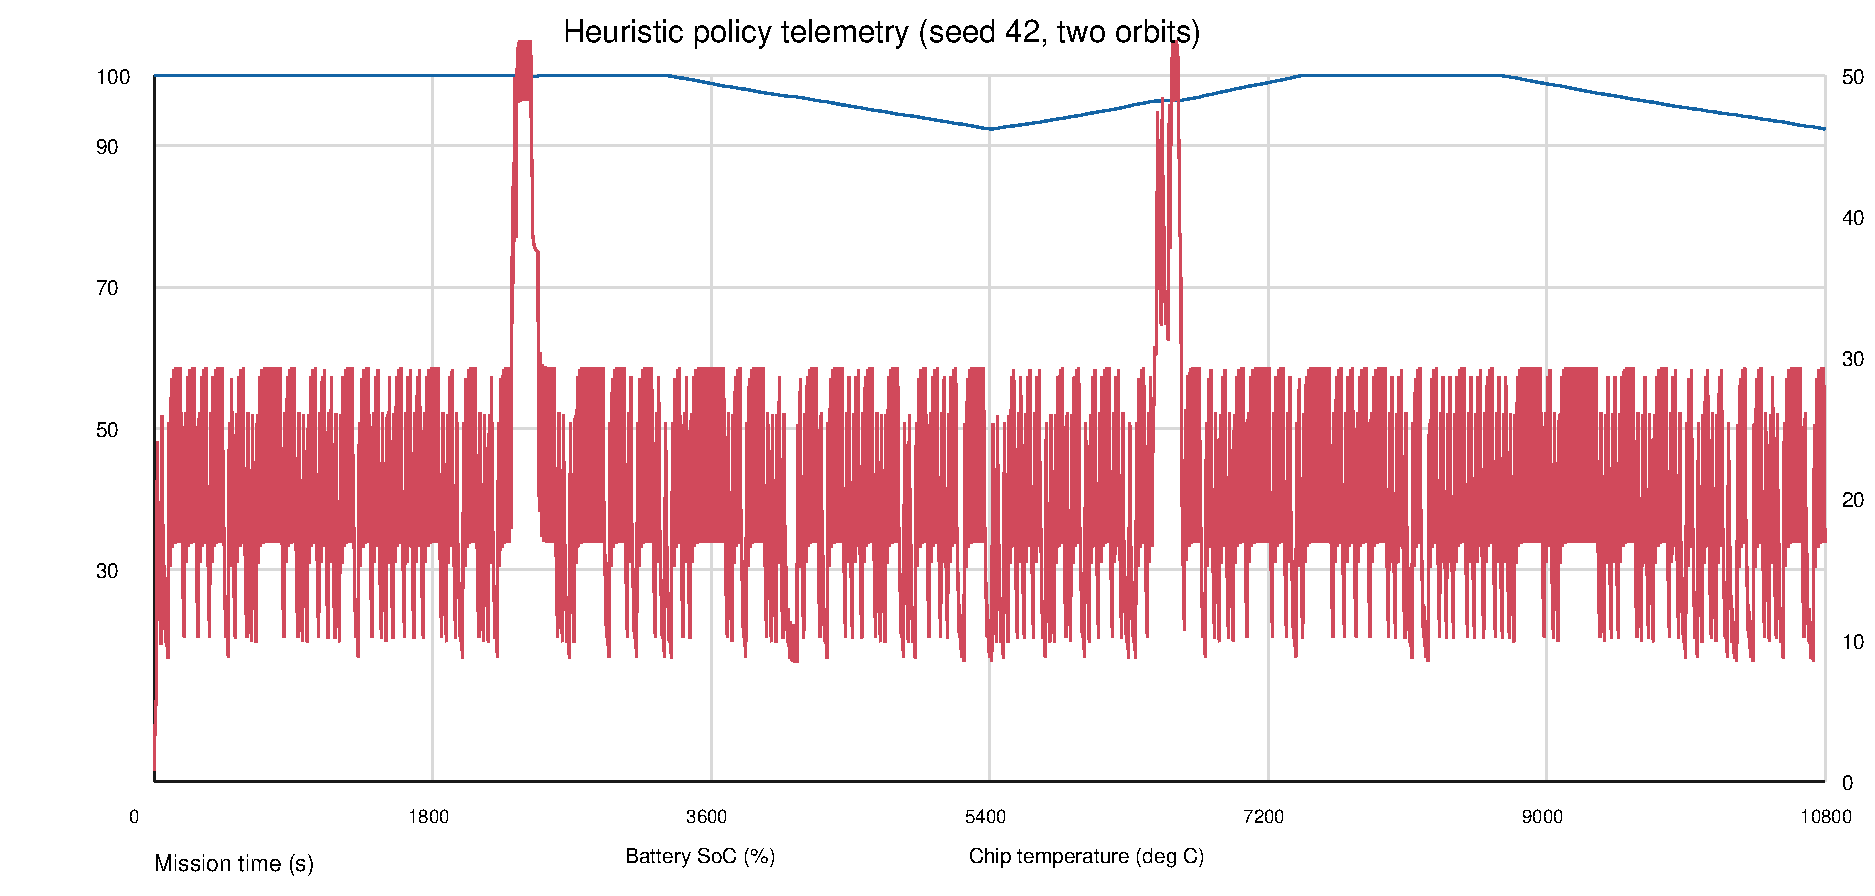
\includegraphics[width=\columnwidth]{../../results/figures/orbit_telemetry.pdf}
\caption{Heuristic trajectory over two orbits (seed 42). Temperature exceeds the 50$^\circ$C throttle threshold.}
\label{fig:telemetry}
\end{figure}

This is a single-policy characterization. The current codebase does not implement the claimed transmit-all comparison, Lyapunov scheduler, or MILP oracle; comparative policy results are future work.

\subsection{Phase 3 Validation Plan}
Phase~3 development will: (1) train a MaskablePPO agent in \textit{simulation/rl\_env.py}; (2) integrate the Lyapunov safety filter to bound RL proposals; (3) compute the MILP oracle ceiling; and (4) stress-test under solar flare SEU bursts ($p_{\text{seu}} = 10^{-3}$) and degraded battery packs ($60\text{ Wh}$).

\section{Conclusion}
We report a reproducible five-seed, four-orbit characterization of the implemented heuristic. The measured decision-quality ratio is 0.0283 on the current simulator workload. The two-orbit trace also exposes a thermal-model limitation: simulated temperature can exceed the 50$^\circ$C throttling threshold. Future work includes comparative baselines, a calibrated thermal model with a hard safety guard, and implementation of Lyapunov and oracle schedulers.

\bibliographystyle{IEEEtran}
\begin{thebibliography}{00}
\bibitem{denby2020orbital} B. Denby and B. Lucia, ``Orbital Edge Computing: Machine Inference in Space,'' \textit{IEEE Micro}, vol. 40, no. 1, pp. 7--15, Jan.--Feb. 2020.
\bibitem{pfandzelter2024trabant} T. Pfandzelter, N. Bauer, A. Leis, C. Perdrizet, F. Trautwein, T. Schirmer, O. Abboud, and D. Bermbach, ``Trabant: A Serverless Architecture for Multi-Tenant Orbital Edge Computing,'' arXiv:2504.08337, 2025.
\bibitem{zhang2023satellite} C. Wang, Y. Zhang, Q. Li, A. Zhou, and S. Wang, ``Satellite Computing: A Case Study of Cloud-Native Satellites,'' arXiv:2307.08530, 2023.
\bibitem{chen2025spaceai} Z. Wang, ``Space AI: Leveraging Artificial Intelligence for Space to Improve Life on Earth,'' \textit{arXiv:2512.22399}, 2025.
\bibitem{duggan2025advancing} A. Duggan, B. Andrade, and H. Afli, ``Advancing Earth Observation: A Survey on AI-Powered Image Processing in Satellites,'' arXiv:2501.12030, 2025.
\bibitem{lentaris2024fpga} P. Antunes and A. Podobas, ``FPGA-Based Neural Network Accelerators for Space Applications: A Survey, arXiv:2504.16173, 2025 (version 3, June 2026).
\bibitem{denby2025when} R. Thummala and G. Falco, ``When to Compute in Space,'' \textit{arXiv:2512.17054}, 2025.
\bibitem{suncatcher2025} B. Agüera y Arcas et al., ``Towards a Future Space-Based, Highly Scalable AI Infrastructure System Design (Project Suncatcher),'' \textit{arXiv:2511.19468}, 2025.
\bibitem{iastam2026spec} IEEE Industry Applications Society, ``IASTAM 6.0 Technical Challenge Specification Book: Track 1 AI \& Onboard Computing,'' IEEE IAS Tunisia Annual Meeting, 2026.
\bibitem{neely2010stochastic} M. J. Neely, \textit{Stochastic Network Optimization with Application to Communication and Queueing Systems}, Morgan \& Claypool Publishers, 2010.
\end{thebibliography}

\end{document}
